%%
%% This is file `sample-sigconf.tex',
%% generated with the docstrip utility.
%%
%% The original source files were:
%%
%% samples.dtx  (with options: `all,proceedings,bibtex,sigconf')
%% 
%% IMPORTANT NOTICE:
%% 
%% For the copyright see the source file.
%% 
%% Any modified versions of this file must be renamed
%% with new filenames distinct from sample-sigconf.tex.
%% 
%% For distribution of the original source see the terms
%% for copying and modification in the file samples.dtx.
%% 
%% This generated file may be distributed as long as the
%% original source files, as listed above, are part of the
%% same distribution. (The sources need not necessarily be
%% in the same archive or directory.)
%%
%%
%% Commands for TeXCount
%TC:macro \cite [option:text,text]
%TC:macro \citep [option:text,text]
%TC:macro \citet [option:text,text]
%TC:envir table 0 1
%TC:envir table* 0 1
%TC:envir tabular [ignore] word
%TC:envir displaymath 0 word
%TC:envir math 0 word
%TC:envir comment 0 0
%%
%% The first command in your LaTeX source must be the \documentclass
%% command.
%%
%% For submission and review of your manuscript please change the
%% command to \documentclass[manuscript, screen, review]{acmart}.
%%
%% When submitting camera ready or to TAPS, please change the command
%% to \documentclass[sigconf]{acmart} or whichever template is required
%% for your publication.
%%
%%
\documentclass[sigconf]{acmart}
%%
%% \BibTeX command to typeset BibTeX logo in the docs
\AtBeginDocument{%
  \providecommand\BibTeX{{%
    Bib\TeX}}}

%% Rights management information.  This information is sent to you
%% when you complete the rights form.  These commands have SAMPLE
%% values in them; it is your responsibility as an author to replace
%% the commands and values with those provided to you when you
%% complete the rights form.
\setcopyright{acmlicensed}
\copyrightyear{2025}
\acmYear{2025}
\acmDOI{XXXXXXX.XXXXXXX}
%% These commands are for a PROCEEDINGS abstract or paper.
\acmConference[Conference acronym 'XX]{Make sure to enter the correct
  conference title from your rights confirmation email}{June 03--05,
  2025}{Woodstock, NY}
%%
%%  Uncomment \acmBooktitle if the title of the proceedings is different
%%  from ``Proceedings of ...''!
%%
%%\acmBooktitle{Woodstock '18: ACM Symposium on Neural Gaze Detection,
%%  June 03--05, 2018, Woodstock, NY}
\acmISBN{978-1-4503-XXXX-X/2025/05}
\raggedbottom % 防止均匀分布垂直空白


%%
%% Submission ID.
%% Use this when submitting an article to a sponsored event. You'll
%% receive a unique submission ID from the organizers
%% of the event, and this ID should be used as the parameter to this command.
%%\acmSubmissionID{123-A56-BU3}

%%
%% For managing citations, it is recommended to use bibliography
%% files in BibTeX format.
%%
%% You can then either use BibTeX with the ACM-Reference-Format style,
%% or BibLaTeX with the acmnumeric or acmauthoryear sytles, that include
%% support for advanced citation of software artefact from the
%% biblatex-software package, also separately available on CTAN.
%%
%% Look at the sample-*-biblatex.tex files for templates showcasing
%% the biblatex styles.
%%

%%
%% The majority of ACM publications use numbered citations and
%% references.  The command \citestyle{authoryear} switches to the
%% "author year" style.
%%
%% If you are preparing content for an event
%% sponsored by ACM SIGGRAPH, you must use the "author year" style of
%% citations and references.
%% Uncommenting
%% the next command will enable that style.
%%\citestyle{acmauthoryear}


%%
%% end of the preamble, start of the body of the document source.
\begin{document}

%%
%% The "title" command has an optional parameter,
%% allowing the author to define a "short title" to be used in page headers.
\title{Contrastive Learning for Time-Series Anomaly Detection in IoT}

%%
%% The "author" command and its associated commands are used to define
%% the authors and their affiliations.
%% Of note is the shared affiliation of the first two authors, and the
%% "authornote" and "authornotemark" commands
%% used to denote shared contribution to the research.
\author{QiPingZhi Xiao}
\email{m202472199@hust.edu.cn}
\affiliation{%
  \institution{%
    School of Cyber Science and Engineering, Huazhong University of Science and Technology
  }
  \city{Wuhan}
  \state{Hubei}
  \country{China}
}
% \author{Ben Trovato}
% \authornote{Both authors contributed equally to this research.}
% \email{trovato@corporation.com}
% \orcid{1234-5678-9012}
% \author{G.K.M. Tobin}
% \authornotemark[1]
% \email{webmaster@marysville-ohio.com}
% \affiliation{%
%   \institution{Institute for Clarity in Documentation}
%   \city{Dublin}
%   \state{Ohio}
%   \country{USA}
% }

% \author{Lars Th{\o}rv{\"a}ld}
% \affiliation{%
%   \institution{The Th{\o}rv{\"a}ld Group}
%   \city{Hekla}
%   \country{Iceland}}
% \email{larst@affiliation.org}

% \author{Valerie B\'eranger}
% \affiliation{%
%   \institution{Inria Paris-Rocquencourt}
%   \city{Rocquencourt}
%   \country{France}
% }

% \author{Aparna Patel}
% \affiliation{%
%  \institution{Rajiv Gandhi University}
%  \city{Doimukh}
%  \state{Arunachal Pradesh}
%  \country{India}}

% \author{Huifen Chan}
% \affiliation{%
%   \institution{Tsinghua University}
%   \city{Haidian Qu}
%   \state{Beijing Shi}
%   \country{China}}

% \author{Charles Palmer}
% \affiliation{%
%   \institution{Palmer Research Laboratories}
%   \city{San Antonio}
%   \state{Texas}
%   \country{USA}}
% \email{cpalmer@prl.com}

% \author{John Smith}
% \affiliation{%
%   \institution{The Th{\o}rv{\"a}ld Group}
%   \city{Hekla}
%   \country{Iceland}}
% \email{jsmith@affiliation.org}

% \author{Julius P. Kumquat}
% \affiliation{%
%   \institution{The Kumquat Consortium}
%   \city{New York}
%   \country{USA}}
% \email{jpkumquat@consortium.net}

%%
%% By default, the full list of authors will be used in the page
%% headers. Often, this list is too long, and will overlap
%% other information printed in the page headers. This command allows
%% the author to define a more concise list
%% of authors' names for this purpose.
\renewcommand{\shortauthors}{QiPingZhi Xiao}

%%
%% The abstract is a short summary of the work to be presented in the
%% article.
\begin{abstract}
  The Internet of Things (IoT) generates vast time-series data from interconnected devices, 
where anomalies may indicate critical failures, cyber threats, or operational inefficiencies. 
Despite advances in anomaly detection, challenges persist due to complex temporal patterns, 
scarcity of labeled anomalies, and intricate dependencies in multivariate data. 
Traditional unsupervised methods often fail to capture temporal dynamics or suffer from high 
computational costs, while deep learning approaches struggle with representation consistency across domains. 
In this work proposes a Time-Frequency Transformer Model for multivariate 
time-series anomaly detection, leveraging dual-path reconstruction in time and frequency domains to exploit the 
inherent instability of anomalous patterns. Key innovations include: (1) a cross-domain reconstruction error analysis 
to enhance anomaly discrimination, (2) a multi-perspective contrastive learning mechanism for robust 
feature representation, and (3) a hierarchical loss aggregation strategy that computes stage-wise reconstruction 
errors for improved sensitivity.Extensive experiments on univariate and multivariate datasets demonstrate that 
our model surpasses state-of-the-art baselines, achieving superior detection performance. 
The framework’s ability to integrate temporal and spectral insights offers broad applicability in IoT domains, 
from infrastructure monitoring to predictive maintenance.
\end{abstract}

%%
%% The code below is generated by the tool at http://dl.acm.org/ccs.cfm.
%% Please copy and paste the code instead of the example below.
%%
% \begin{CCSXML}
% <ccs2012>
%  <concept>
%   <concept_id>00000000.0000000.0000000</concept_id>
%   <concept_desc>Do Not Use This Code, Generate the Correct Terms for Your Paper</concept_desc>
%   <concept_significance>500</concept_significance>
%  </concept>
%  <concept>
%   <concept_id>00000000.00000000.00000000</concept_id>
%   <concept_desc>Do Not Use This Code, Generate the Correct Terms for Your Paper</concept_desc>
%   <concept_significance>300</concept_significance>
%  </concept>
%  <concept>
%   <concept_id>00000000.00000000.00000000</concept_id>
%   <concept_desc>Do Not Use This Code, Generate the Correct Terms for Your Paper</concept_desc>
%   <concept_significance>100</concept_significance>
%  </concept>
%  <concept>
%   <concept_id>00000000.00000000.00000000</concept_id>
%   <concept_desc>Do Not Use This Code, Generate the Correct Terms for Your Paper</concept_desc>
%   <concept_significance>100</concept_significance>
%  </concept>
% </ccs2012>
% \end{CCSXML}

% \ccsdesc[500]{Do Not Use This Code~Generate the Correct Terms for Your Paper}
% \ccsdesc[300]{Do Not Use This Code~Generate the Correct Terms for Your Paper}
% \ccsdesc{Do Not Use This Code~Generate the Correct Terms for Your Paper}
% \ccsdesc[100]{Do Not Use This Code~Generate the Correct Terms for Your Paper}

%%
%% Keywords. The author(s) should pick words that accurately describe
%% the work being presented. Separate the keywords with commas.
\keywords{Contrastive learning, time Series, anomaly Detection, internet of Things}
%% A "teaser" image appears between the author and affiliation
%% information and the body of the document, and typically spans the
%% page.
% \begin{teaserfigure}
%   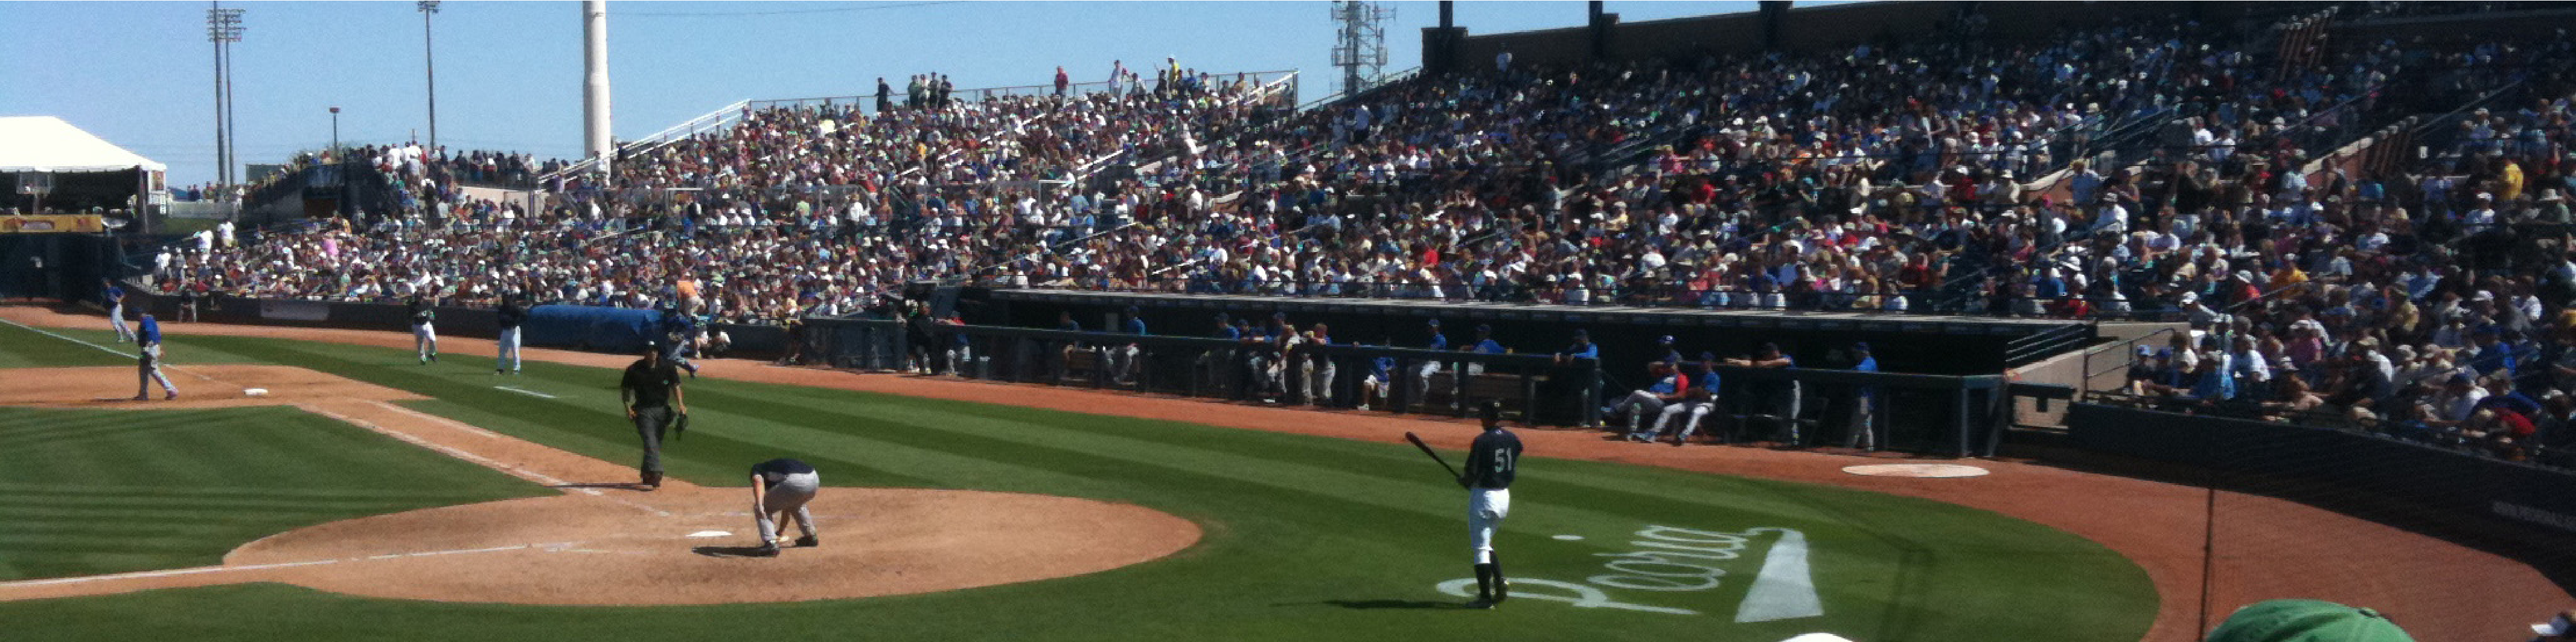
\includegraphics[width=\textwidth]{sampleteaser}
%   \caption{Seattle Mariners at Spring Training, 2010.}
%   \Description{Enjoying the baseball game from the third-base
%   seats. Ichiro Suzuki preparing to bat.}
%   \label{fig:teaser}
% \end{teaserfigure}

\received{20 February 2025}
\received[revised]{12 March 2025}
\received[accepted]{5 June 2025}

%%
%% This command processes the author and affiliation and title
%% information and builds the first part of the formatted document.
\maketitle

\section{Introduction}

The Internet of Things (IoT) has become a cornerstone of modern industry and everyday life, 
enabling seamless connectivity among computing devices, mechanical systems, and
digital machines. These interconnected devices, each assigned unique identifiers,
autonomously collect and transmit data across networks, generating time-series
signals that reflect system dynamics. Despite their widespread adoption,
IoT systems remain susceptible to various security risks and operational vulnerabilities.

Anomalies in IoT data can arise from unexpected technical malfunctions, human errors,
or malicious intrusions, potentially disrupting system stability and leading to service failures.
For instance, in a distributed server environment, real-time monitoring of performance metrics—such as user traffic,
CPU utilization, and memory consumption—is essential. The presence of outliers in these metrics may signal cyber
threats or system inefficiencies, underscoring the importance of
anomaly detection in maintaining operational integrity and cybersecurity.

Similarly, in industrial IoT applications, sensor anomalies often indicate critical
failures requiring immediate intervention. Consider a water distribution (WADI) system 
equipped with sensors to monitor water quality. Anomalous readings during disinfection 
could suggest hazardous chlorine levels, necessitating rapid alerts to prevent 
health risks. Thus, time-series anomaly detection has emerged as a vital tool across IoT 
domains, including infrastructure management, health monitoring, 
and predictive maintenance.

Although anomaly detection techniques have broad applicability, 
achieving precise anomaly identification in complex time-series data 
still faces several critical challenges.First, time-series data often 
exhibit multiple intricate patterns, including but not limited to 
seasonality, trends, and periodicity. Effectively distinguishing these 
patterns while accurately detecting anomalies within them remains 
a significant difficulty. Second, anomalous events are inherently rare 
in real-world scenarios, making it challenging to obtain sufficient high-quality 
labeled training data. This scarcity hinders the development of robust 
supervised learning models. Third, the temporal and feature-wise 
dependencies embedded in time-series data must be carefully considered. 
The ability of an anomaly detection model to properly capture and 
process these dependencies is crucial for reliable performance.

Anomalous data exhibits two inherent characteristics that make detection 
challenging: its scarcity compared to normal data and its concealment within 
large volumes of regular observations. To address the scarcity of 
both labeled anomalies and anomaly examples, researchers have developed 
numerous unsupervised learning approaches.These conventional unsupervised 
methods employ diverse strategies for distinguishing normal patterns from 
anomalies and have demonstrated reasonable effectiveness. However, they 
suffer from three critical limitations: (1) failure to account for temporal 
dependencies in time-series data, (2) high computational complexity when 
processing large-scale datasets, and (3) heightened sensitivity to parameter 
configurations. These constraints ultimately restrict their detection 
performance and practical applicability.Unsupervised approaches extend beyond 
conventional machine learning methods, with numerous deep learning models now employing 
unsupervised techniques for time-series anomaly detection. These 
methods share a common underlying principle: they exploit dual perspectives 
to create significant divergence between normal and anomalous data in either feature 
space representation or reconstruction outcomes, thereby enabling effective anomaly discrimination.

Inspired by these approaches, we observe that normal samples maintain representation 
consistency during multi-perspective feature learning and reconstruction, 
while anomalous samples exhibit unstable cross-dimensional representations due to 
their inherent pattern instability, making it difficult to achieve consistent or 
approximate reconstruction results. Furthermore, according to the uncertainty principle 
of time series representation, anomaly data that demonstrates significant representational 
advantages in either the time or frequency domain typically fails to maintain comparable 
performance in the corresponding counterpart domain.Building upon these insights, 
this paper proposes a Time-Frequency Transformer Based Model for Multivariate Time Series Anomaly Detection. 
The model simultaneously performs feature representation and reconstruction in both 
time and frequency domains, effectively capturing anomalies by comparing the discrepancies between 
reconstruction results across these dual domains.Notably, our approach introduces 
a significant improvement over conventional methods that only compute reconstruction loss 
at the final stage. Instead, we implement a stage-wise loss aggregation mechanism that 
calculates and averages the reconstruction loss at each processing stage. This enhancement 
has demonstrably improved the model's overall performance.

In summary, the contributions of our work are as follows.
\begin{itemize}
\item We propose a novel anomaly detection framework that effectively integrates 
time-domain and frequency-domain information. The model performs dual-path reconstruction 
from both temporal and spectral perspectives, enabling accurate discrimination between 
normal and anomalous patterns through cross-domain reconstruction error analysis.
\item We develop a multi-perspective contrastive learning mechanism that systematically 
compares temporal and spectral representations. This approach facilitates comprehensive 
exploration of feature extraction across different data modalities.
\item We introduce a hierarchical reconstruction loss aggregation strategy that computes 
and averages mean squared errors at each processing stage. This novel loss computation 
method significantly enhances the model's detection capability by capturing multi-scale reconstruction discrepancies.
\item Extensive experimental results demonstrate that our model outperforms existing 
baseline methods across multiple univariate and multivariate datasets, establishing 
new state-of-the-art performance benchmarks.
\end{itemize}

\section{Related Work}

\subsection{Prediction-Based Anomaly Detection Models}

The fundamental principle of prediction-based anomaly detection models involves training 
models on historical data to forecast future values, with anomalies identified through discrepancies 
between predicted and observed time series. Data points exhibiting deviations beyond 
a predefined threshold are classified as anomalous.Several notable approaches have advanced this paradigm:
THOC employs multi-scale dilated convolutional recurrent neural networks with skip connections to capture 
temporal dynamics, coupled with a hierarchical clustering process that generates multiple hyperspheres 
to define its novel Multiscale Vector Data Description objective \cite{shen2020timeseries}.
Hundman et al. developed an LSTM-based forecasting model integrated with an unsupervised, 
parameter-free thresholding technique for monitoring anomalies in spacecraft telemetry data \cite{hundman2018detecting}.
Ren et al. designed a hybrid algorithm combining Spectral Residual (SR) analysis with Convolutional 
Neural Networks (CNNs) for anomaly detection in Microsoft service operations \cite{ren2019time}.
Ahmad et al. proposed a Hierarchical Temporal Memory (HTM) model, an unsupervised online sequence 
memory algorithm for real-time anomaly detection in data streams \cite{ahmad2017unsupervised}.
While prediction-based methods demonstrate strong performance in modeling temporal progression, 
they face two critical limitations: 
(1) susceptibility to noise and artifacts in historical training data, 
and (2) potential failure to detect non-conventional anomalies due to their rigid definition of deviation patterns.

\subsection{Reconstruction-Based Anomaly Detection Models}

Reconstruction-based anomaly detection models typically employ an encoder-decoder architecture, 
where the encoder maps raw time series into a latent space representation and the decoder attempts 
to reconstruct the original sequence from this compressed form. Data points exhibiting reconstruction 
errors exceeding a predetermined threshold are identified as anomalies.
The Variational Autoencoder (VAE) represents a fundamental reconstruction-based model, 
originally proposed as a directed probabilistic graphical model for efficient approximate inference and learning \cite{kingma2013auto}. 
VAEs have found widespread application in various domains including denoising, data compression, and anomaly detection.
Another notable approach, DAGMM (Deep Autoencoding Gaussian Mixture Model), performs unsupervised anomaly detection 
by generating low-dimensional representations and reconstruction errors through deep autoencoders \cite{zong2018deep}.
Despite the prevalence of VAEs in reconstruction-based methods, significant variations exist in encoder design:
Wang et al. employed simple Multilayer Perceptrons (MLPs) and Recurrent Neural Networks (RNNs) as encoders for air quality anomaly detection \cite{wang2019quality}.
Zhang et al. developed a more sophisticated approach incorporating time-frequency analysis, using Temporal 
Convolutional Networks (TCNs) as primary encoder components to separately reconstruct temporal and spectral features, 
along with trend and residual components \cite{zhang2022tfad}.
While these methods have demonstrated promising results, most existing approaches focus exclusively on time-domain modeling, 
neglecting the potentially valuable information contained in frequency-domain representations. 
This limitation may restrict their ability to detect certain types of anomalies that manifest more clearly in the spectral domain.

\subsection{Transformer-Based Anomaly Detection Models}

Since its inception, the Transformer architecture has achieved remarkable success in natural 
language processing and has subsequently been widely adopted in computer vision applications. 
Recently, an increasing number of Transformer-based models are being applied to time series tasks.
Several notable Transformer-based approaches have advanced time series anomaly detection:
The Anomaly Transformer introduces a novel Anomaly-Attention mechanism that simultaneously models prior 
associations and sequential relationships to capture association discrepancies, effectively distinguishing 
between normal and anomalous patterns \cite{xu2021anomaly}.
Nam et al. proposed a nested window approach combining external and internal windows to align anomaly 
scores from time-domain and frequency-domain reconstructions, enabling more precise identification of abnormal pattern boundaries \cite{nam2024breaking}.
TranAD developed a two-stage encoder-decoder architecture stabilized through adversarial training, 
significantly improving reconstruction performance \cite{tuli2022tranad}.
AnomalyBert addressed the scarcity of real-world anomalies by proposing four distinct degradation methods to synthesize anomalous patterns, 
effectively augmenting training data for rare anomaly cases \cite{jeong2023anomalybert}.

\subsection{Time Series Anomaly Detection Models Based on Time Domain Analysis}

Time series data typically exhibit multiple complex temporal patterns, 
where decomposition techniques play a crucial role in extracting distinct components to facilitate deeper 
understanding and analysis of temporal characteristics. Recent advances have demonstrated the 
effectiveness of decomposition-based approaches in anomaly detection:
Lei et al. developed a novel deep learning framework that 
integrates time series decomposition with spectral analysis for enhanced anomaly detection \cite{lei2023novel}.
Autoformer introduced an innovative inner decomposition block that endows deep forecasting 
models with inherent progressive decomposition capabilities \cite{wu2021autoformer}.
MICN validated the necessity and effectiveness of separately modeling complex temporal patterns 
through multi-scale kernel decomposition of input data \cite{wang2023micn}.
TFDNet proposed a specialized sequence decomposition method for long-horizon time series, 
significantly improving both prediction efficiency and robustness \cite{luo2025tfdnet}.
D3R presented a dynamic decomposition approach for long-period multivariate time series, 
effectively utilizing external information to overcome limitations of local sliding windows \cite{wang2023drift}.

\section{COMMENTS}

\subsection{Excessively long declarative sentences}

The first comment addresses the issue of overly long declarative sentences (Figure 1). 
I think The sentence is too lengthy and somewhat confusing in its description. 
It is suggested that it be split into two clearer statements, for example:
By implementing PSI protocols based on different algorithmic schemes, one can better understand them. 
Further, by comparing and analyzing these protocols in different application environments, one can maximize their value.

\begin{figure}[h]
  \centering
  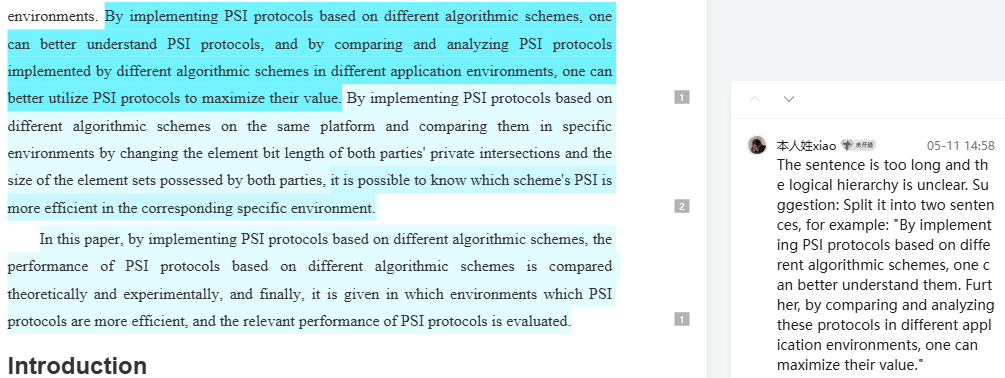
\includegraphics[width=\linewidth]{./picture/excessive_1.png}
  \caption{Excessively long declarative sentences}
  \Description{My Comments on other people's papers.}
\end{figure}

Similarly, the sentence is too long and repeats "cloud environment." (Figure 2) It is suggests that: 
Split it into two sentences, for example: 
PSI protocols have broad applications, including COVID-19 contact tracing, 
address book lookup, and blockchain. Additionally, cloud environments, as a key scenario 
for secure multiparty computation, heavily rely on PSI.

\begin{figure}[h]
  \centering
  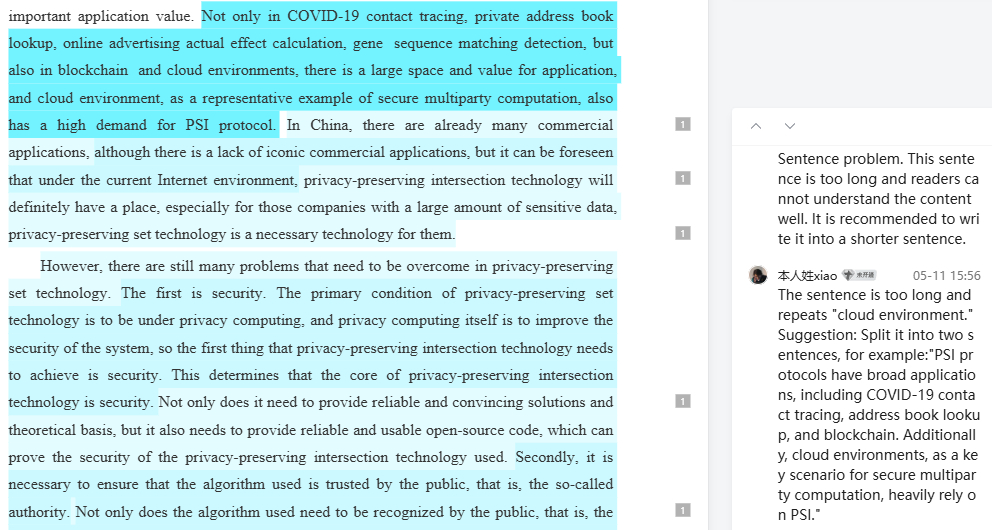
\includegraphics[width=\linewidth]{./picture/excessive_2.png}
  \caption{Excessively long declarative sentences and repeated words}
  \Description{My Comments on other people's papers.}
\end{figure}

\subsection{Passive sentences}

\begin{figure}[h]
  \centering
  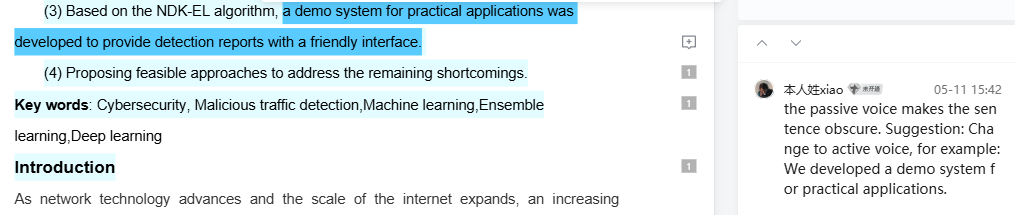
\includegraphics[width=\linewidth]{./picture/passive_2.png}
  \caption{Passive sentences}
  \Description{My Comments on other people's papers.}
\end{figure}

\begin{figure}[h]
  \centering
  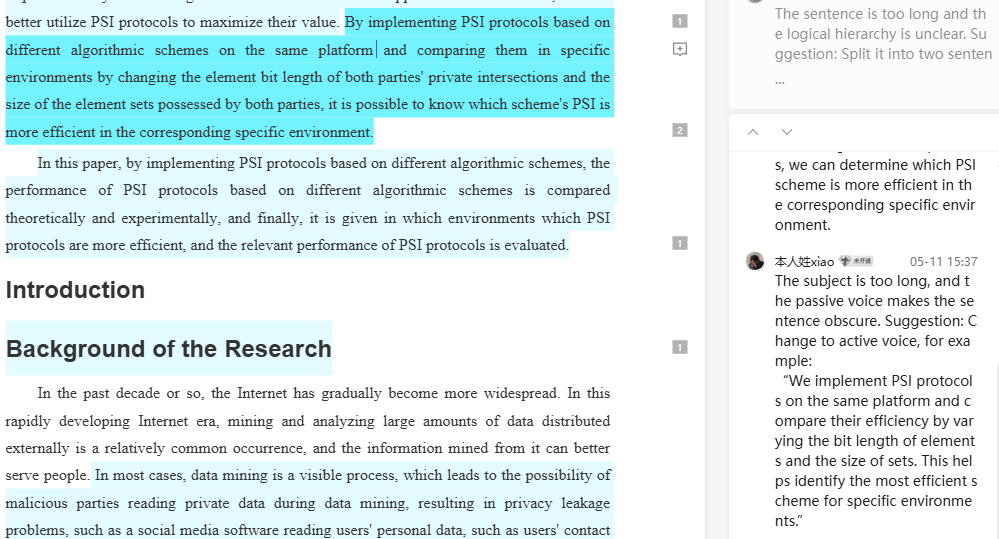
\includegraphics[width=\linewidth]{./picture/passive_1.png}
  \caption{Passive sentences and subject is too long}
  \Description{My Comments on other people's papers.}
\end{figure}

An active sentence is better than a passive sentence, so this sentence (Figure 3) might be better stated this way:
We developed a demo system for practical applications.

Similarly, the recommended way of passive and the subject is too long (Figure 4) is: 
We implement PSI protocols on the same platform and compare their efficiency by varying the bit 
length of elements and the size of sets. This helps identify the most efficient scheme for specific environments.

\subsection{Use of punctuation}

"Different countries and organizations have introduced laws and regulations 
to protect privacy data, and data privacy protection has long been a hot issue."
I think it should replace the comma with a semicolon, i.e., "...privacy data; data privacy protection...", 
as the two parts are independent yet related clauses.

\begin{figure}[h]
  \centering
  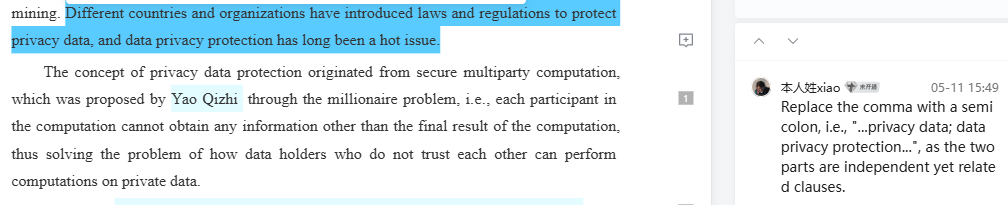
\includegraphics[width=\linewidth]{./picture/punctuation_1.png}
  \caption{Use of punctuation}
  \Description{My Comments on other people's papers.}
\end{figure}

A term "machine learningbased" is missing a hyphen (Figure 6), resulting in incorrect word formation. 
The correct form should be "machine learning-based," so a hyphen needs to be added.

\begin{figure}[h]
  \centering
  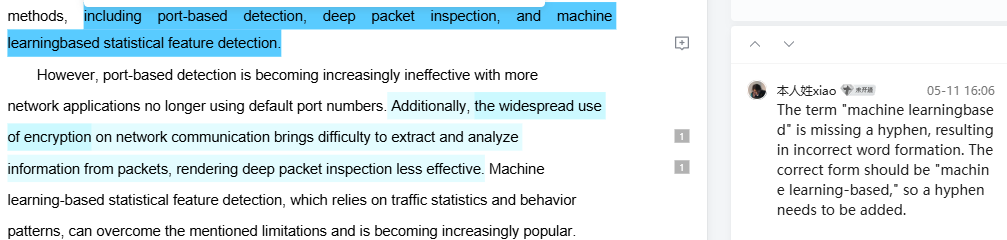
\includegraphics[width=\linewidth]{./picture/punctuation_2.png}
  \caption{Use of punctuation}
  \Description{My Comments on other people's papers.}
\end{figure}

\subsection{Confusing statements}

The logical connection is unclear and confusing (Figure 7), as "through a technology" does not flow coherently with the main clause. 
I recommend rewriting this part of the sentence, for example:
"Although China lacks iconic commercial applications of PSI, 
enterprises holding sensitive data urgently need this technology—it enables 
deep data mining while protecting privacy."

\begin{figure}[h]
  \centering
  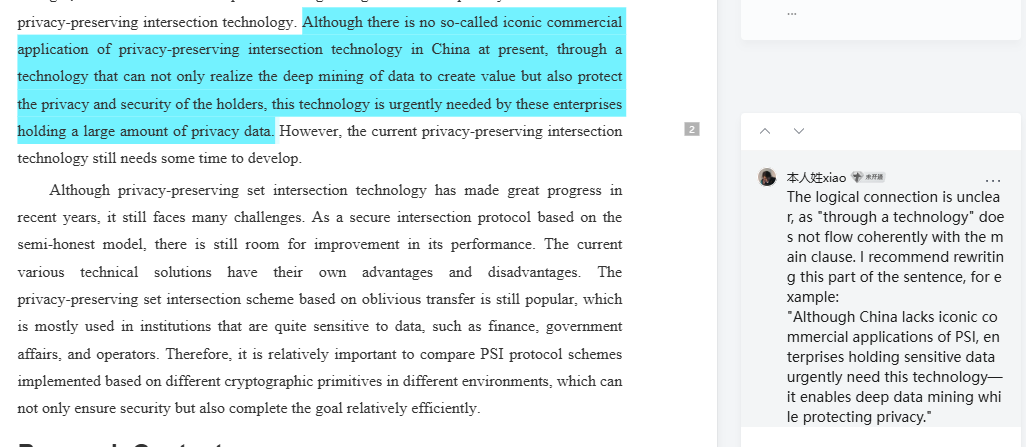
\includegraphics[width=\linewidth]{./picture/confusing_1.png}
  \caption{Confusing statements}
  \Description{My Comments on other people's papers.}
\end{figure}

\subsection{Grammar errors}

There is a grammatical error (Figure 8), 'the' should be added before the sentence.

\begin{figure}[h]
  \centering
  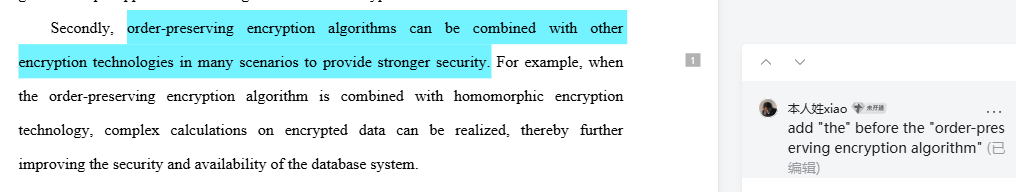
\includegraphics[width=\linewidth]{./picture/grammar_1.png}
  \caption{Grammar errors}
  \Description{My Comments on other people's papers.}
\end{figure}

Similarly, there is a grammatical error (Figure 9), 'the' should be added before the 'database security'.
\begin{figure}[h]
  \centering
  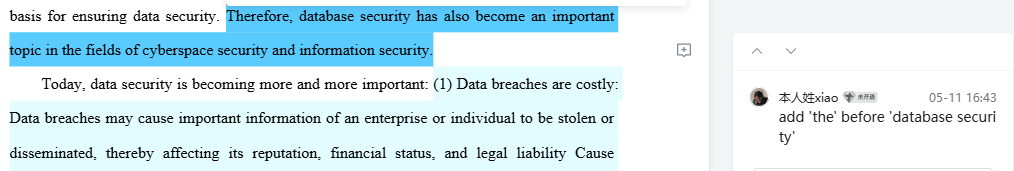
\includegraphics[width=\linewidth]{./picture/grammar_2.png}
  \caption{Grammar errors}
  \Description{My Comments on other people's papers.}
\end{figure}

\subsection{Use of conjuctions}

\begin{figure}[h]
  \centering
  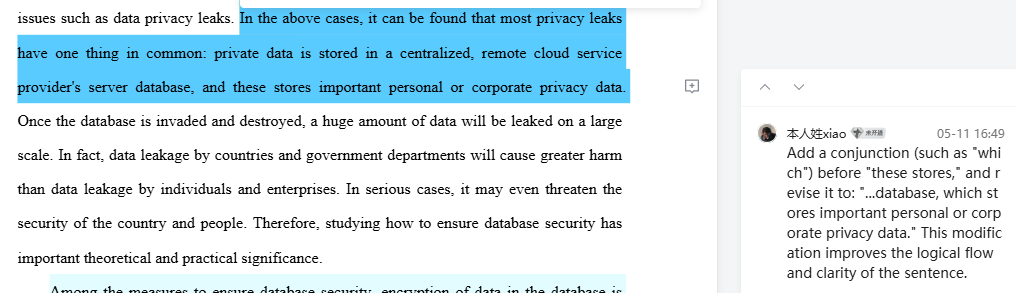
\includegraphics[width=\linewidth]{./picture/conjuction_1.png}
  \caption{Use of conjuctions}
  \Description{My Comments on other people's papers.}
\end{figure}

Logical connection missing (Figure 10): The original sentence reads: 
"In the above cases, it can be found that most privacy leaks have one thing in common: 
private data is stored in a centralized, remote cloud service provider's server database, 
and these stores important personal or corporate privacy data." 
Suggestion: Add a conjunction (such as "which") before "these stores," 
and revise it to: "...database, which stores important personal or corporate privacy data." 
This modification improves the logical flow and clarity of the sentence.

%%
%% The acknowledgments section is defined using the "acks" environment
%% (and NOT an unnumbered section). This ensures the proper
%% identification of the section in the article metadata, and the
%% consistent spelling of the heading.

%%
%% The next two lines define the bibliography style to be used, and
%% the bibliography file.
\bibliographystyle{ACM-Reference-Format}
\bibliography{mywork}


%%
%% If your work has an appendix, this is the place to put it.
\end{document}
\endinput
%%
%% End of file `sample-sigconf.tex'.
